\documentclass{bredelebeamer}

\renewcommand<>{\item}{\beameroriginal\item\vspace{\stretch{.1}}}
\usefonttheme{professionalfonts} % using non standard fonts for beamer
\usefonttheme{serif} % default family is serif
\usepackage[T1]{fontenc}
\usepackage{lmodern}
\usepackage[]{media9}
\setbeamertemplate{itemize/enumerate body begin}{\Large}
\setbeamertemplate{itemize/enumerate subbody begin}{\large}
\setbeamertemplate{itemize/enumerate subsubbody begin}{\large}

\setbeamertemplate{enumerate item}{%
  \usebeamercolor[bg]{item projected}%
  \raisebox{1.5pt}{\colorbox{bg}{\color{fg}\footnotesize\insertenumlabel}}%
}

%%%%%%%%%%%%%%%%%%%%%%%%%%%%%%%%%%%%%%%%%%%%%%%%

\title[Exit Seminar]{\huge Visualizing RNA-seq data: Pertinence, software, and applications}

\author[Lindsay Rutter (ISU)]{\Large Exit Seminar\\ Lindsay Rutter\\ \vspace{9mm} \normalsize \textbf{Program of Study Committee:}\\ Dianne Cook (Major Professor)\\ Amy Toth (Major Professor)\\ Heike Hofmann\\ Daniel Nettleton\\ James Reecy}


\date[May 1, 2018]{\small May 1, 2018}

\subject{Sujet de votre diaporama}
% C'est utilisé dans les métadonnes du PDF

%%%%%%%%%%%%%%%%%%%%%%%%%%%%%%%%%%%%%%%%%%%%%%%%%%%%%%%%%%%%%%%%%%%%%
\begin{document}

\begin{frame}
  \titlepage
\end{frame}

%%%%%%%%%%%%%%%%%%%%%%%%%%%%%%%%%%%% BACKGROUND %%%%%%%%%%%%%%%%%%%%%%%%%%%%%%%%%%%%%
%\section{My Background}

\begin{frame}{My Background}

\begin{itemize}
		\item Education
		\begin{itemize}
		  \item B.S. in Bioengineering\\ \textit{Pennsylvania State University} (2003-2007)
		  \item Major in Bioinformatics and Computational Biology\\ \textit{Iowa State University} (2012-Present)
		  \item Minor in Statistics\\ \textit{Iowa State University} (2012-Present)
		\end{itemize}
		\item Internships
		\begin{itemize}
			\item Nagaoka University of Technology (Summer 2012)
		  \item Okinawa Institute of Science and Technology (Summer 2014)
		  \item MathWorks (Summer 2016)
		  \item After Inc. (Fall 2016)
		  \item Google Summer of Code (Summer 2017)
		  \item GeneLab (Pending - Summer 2018)
		\end{itemize}
	\end{itemize}
\end{frame}


\begin{frame}{Chapter Outline}

\begin{itemize}
		\item \textbf{Chapter 1}\\ 
		Visualization methods for genealogical datasets

		\item \textbf{Chapter 2}\\  
		The case for visualization methods in RNA-seq data analysis

		\item \textbf{Chapter 3}\\
		Software for visualization methods in RNA-seq data analysis
		
		\item \textbf{Chapter 4}\\  
		Gene expression responses to diet quality and viral infection in \textit{Apis mellifera}

	\end{itemize}
\end{frame}

%%%%%%%%%%%%%%%%%%%%%%%%%%%%%%%%% CHAPTER 1 %%%%%%%%%%%%%%%%%%%%%%%%%%%%%
\section{Visualizing genealogy}

\begin{frame}
\begin{center}
\fcolorbox{black}{titleColor}{
\begin{minipage}{\textwidth}
\begin{center}
\huge \textbf{Chapter 1:} Visualization methods for\\
genealogical datasets
\end{center}
\end{minipage}
}
\end{center}
\end{frame}

\begin{frame}{}
\begin{figure}
\centering
\fbox{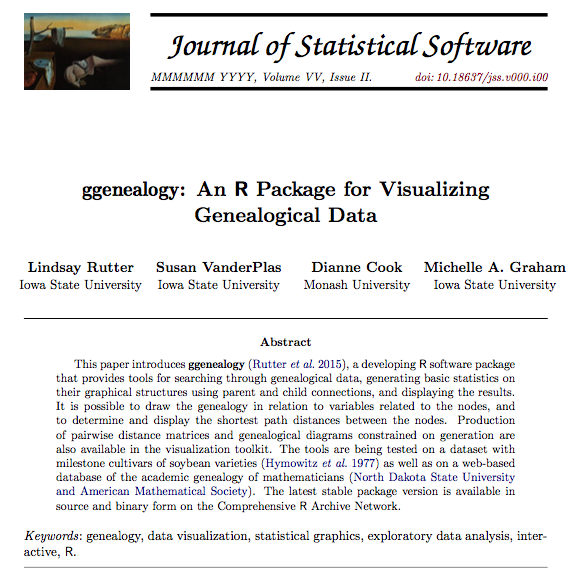
\includegraphics[scale=0.37]{images/JSS.png}}
\end{figure}
\end{frame}

\begin{frame}{}
\begin{figure}
\centering
\fbox{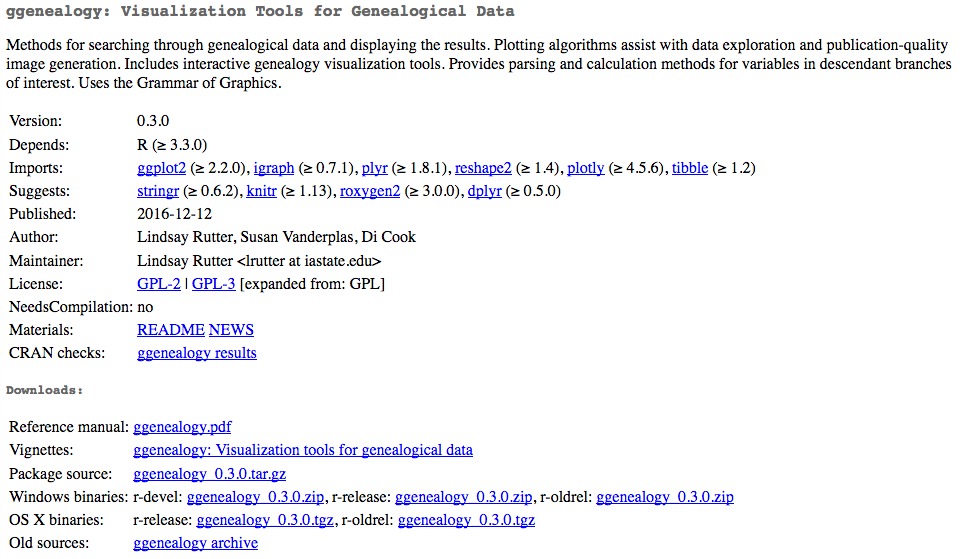
\includegraphics[scale=0.3]{images/ggenealogyCRAN.png}}
\end{figure}
\end{frame}

%%%%%%%%%%%%%%%%%%%%%%%%%%%%%%%%% DEGS %%%%%%%%%%%%%%%%%%%%%%%%%%%%%
\section{Case for Visualizing RNA-seq}

\begin{frame}
\begin{center}
\fcolorbox{black}{titleColor}{
\begin{minipage}{\textwidth}
\begin{center}
\huge \textbf{Chapter 2:} The case for visualization \\
methods in RNA-seq analysis
\end{center}
\end{minipage}
}
\end{center}
\end{frame}

\begin{frame}{}
\begin{figure}
\centering
\fbox{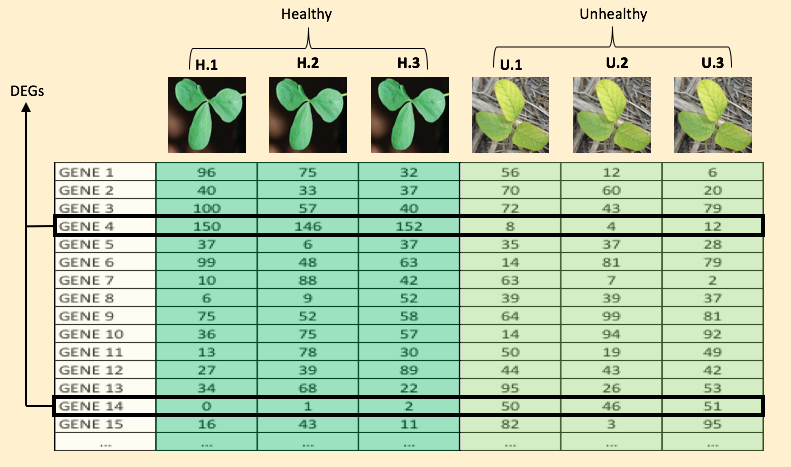
\includegraphics[scale=0.37]{images/RNASeqDesign.png}}
\end{figure}
\end{frame}

\begin{frame}{}
\begin{figure}
\centering
\fbox{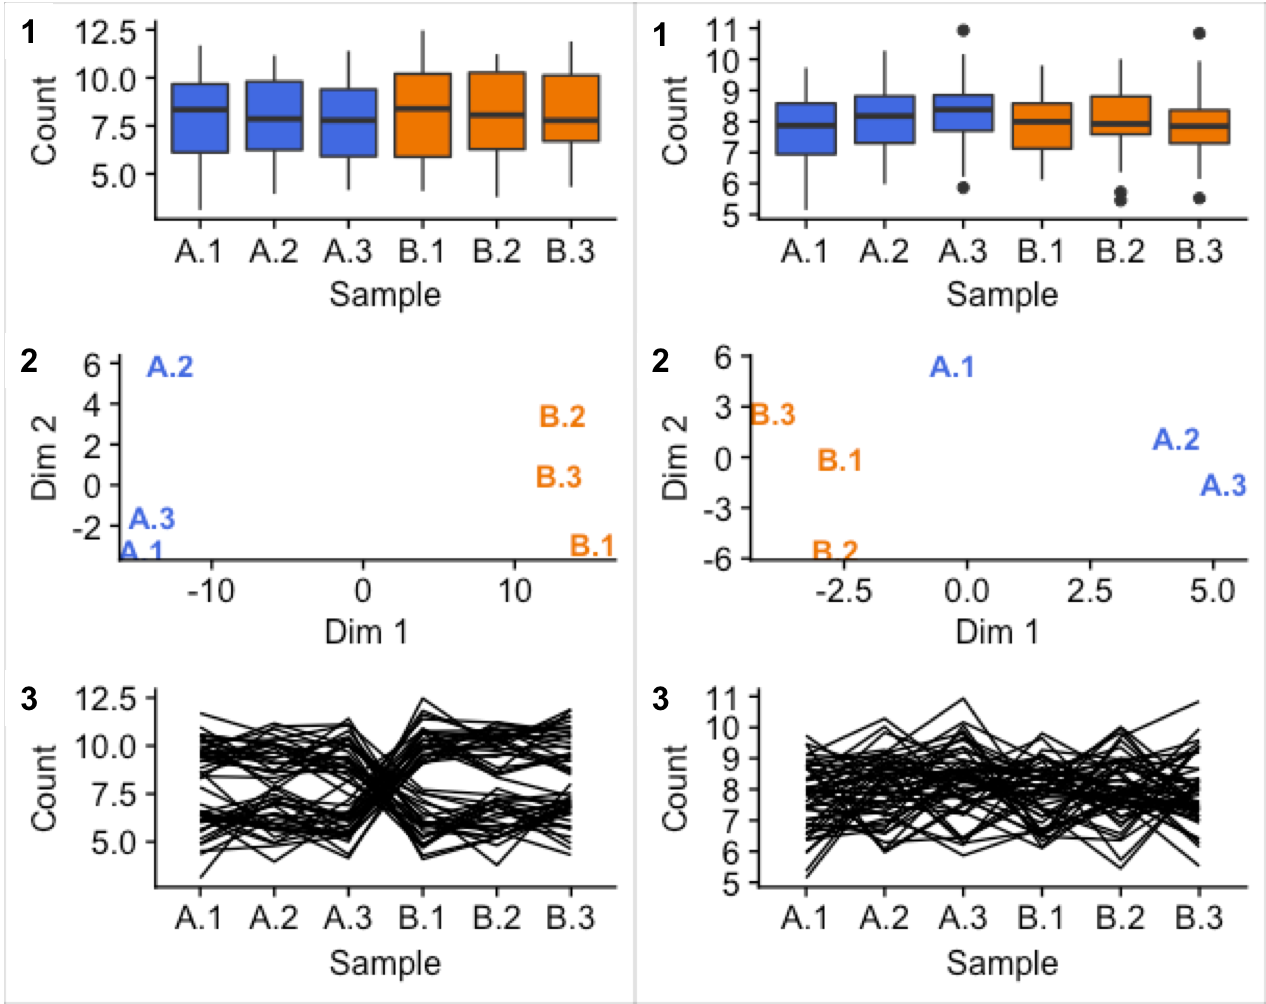
\includegraphics[scale=0.45]{images/mdsBox.png}}
\end{figure}
\end{frame}

\begin{frame}{Three new plotting types}

\begin{itemize}
		\item Parallel coordinate plots\\ 
		\item Scatterplot matrices\\  
		\item repLIcate TREatment ("litre") plots\\
	\end{itemize}
\end{frame}

\begin{frame}{}
\begin{figure}
\centering
\fbox{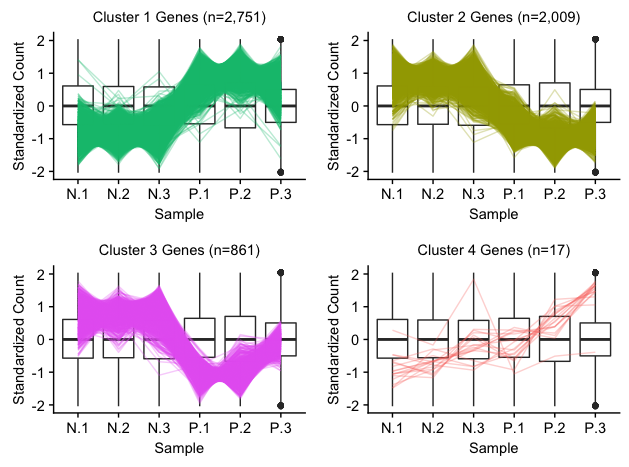
\includegraphics[scale=0.45]{images/sbIRClustersSig.jpg}}
\end{figure}
\end{frame}

\begin{frame}{}
\begin{figure}
\centering
\fbox{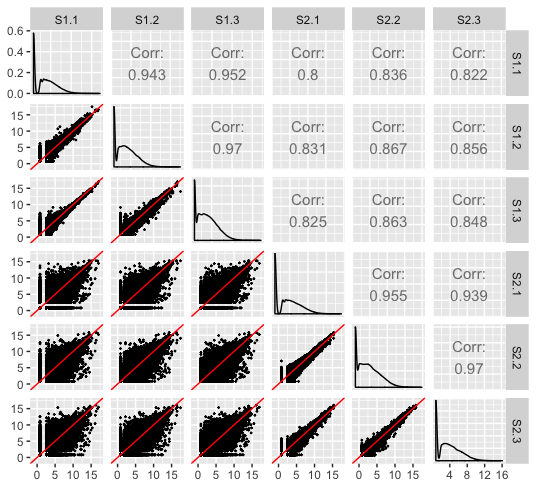
\includegraphics[scale=0.45]{images/sbCNSM.jpg}}
\end{figure}

\centering{https://rnaseqvisualization.shinyapps.io/scatmat}

\end{frame}

\begin{frame}{}
\begin{figure}
\centering
\fbox{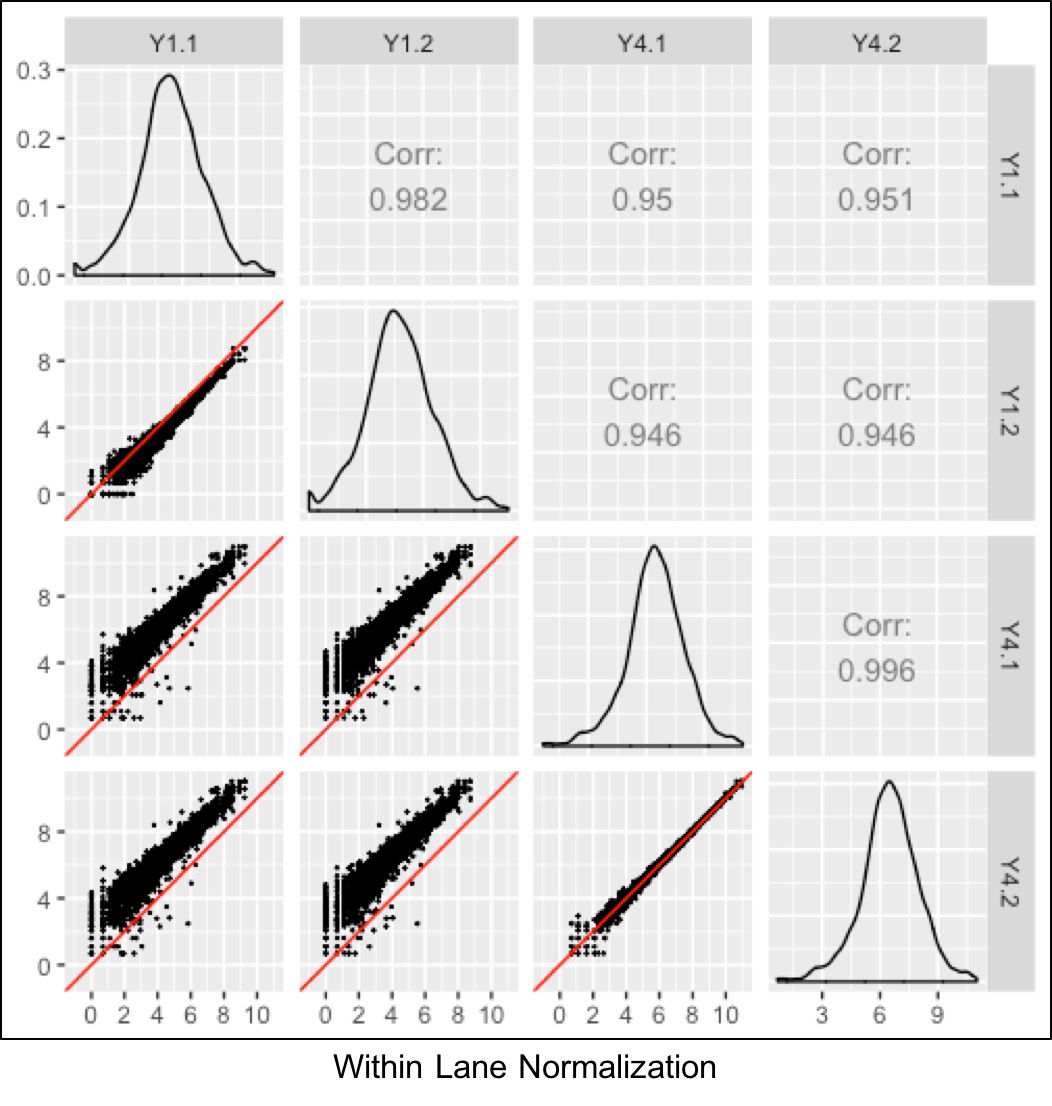
\includegraphics[scale=0.75]{images/yeastWithinBetween.png}}
\end{figure}
\end{frame}

\begin{frame}{}
\begin{figure}
\centering
\fbox{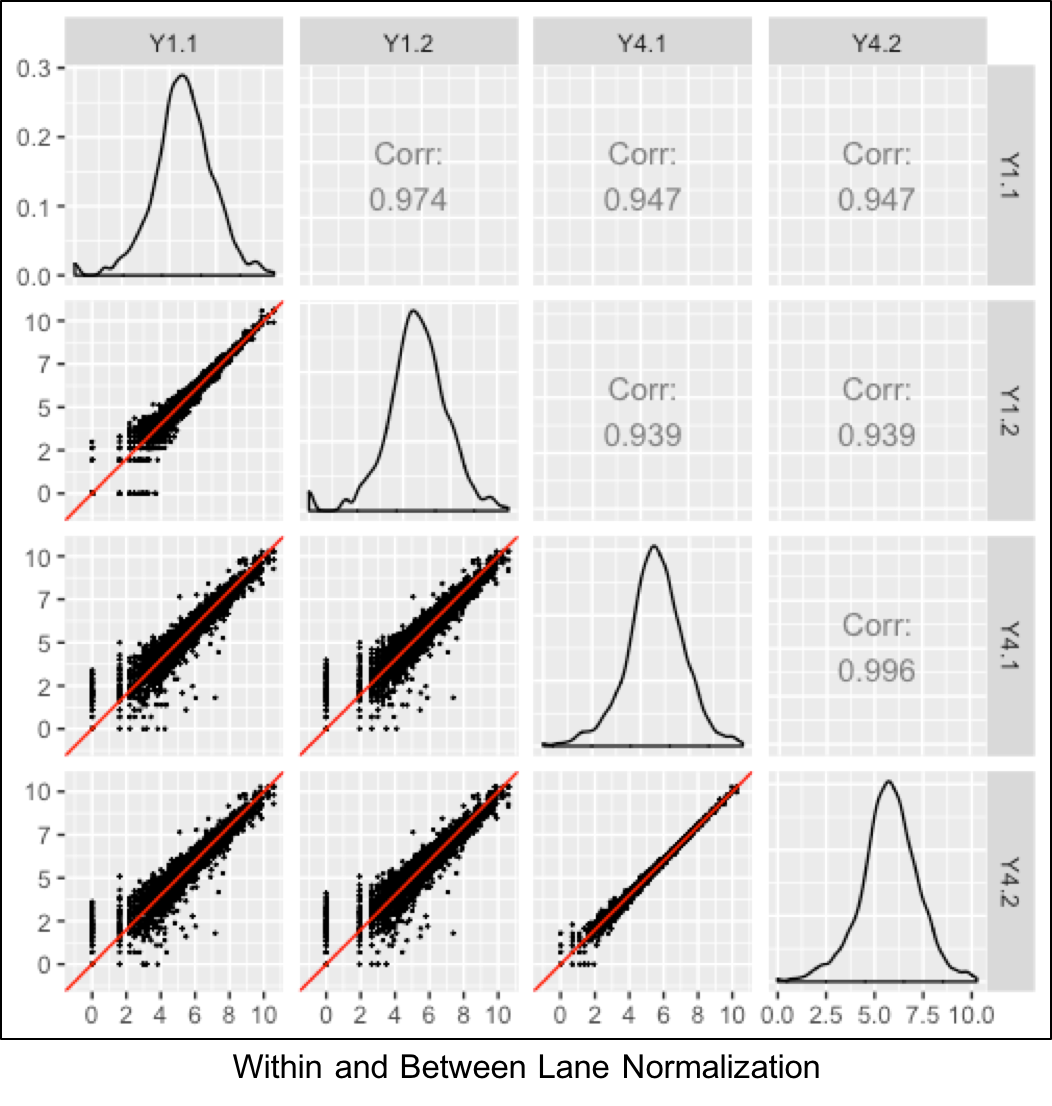
\includegraphics[scale=0.75]{images/yeastWithinBetween2.png}}
\end{figure}
\end{frame}

\begin{frame}{}
\begin{figure}
\centering
\fbox{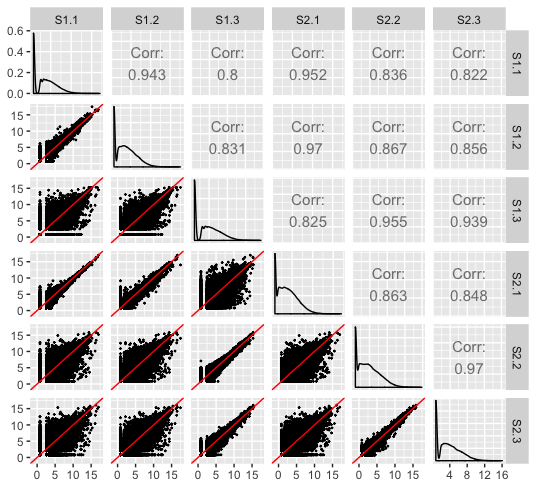
\includegraphics[scale=0.42]{images/sbCNSwitchedSM.jpg}}
\end{figure}
\end{frame}

\begin{frame}{}
\begin{figure}
\centering
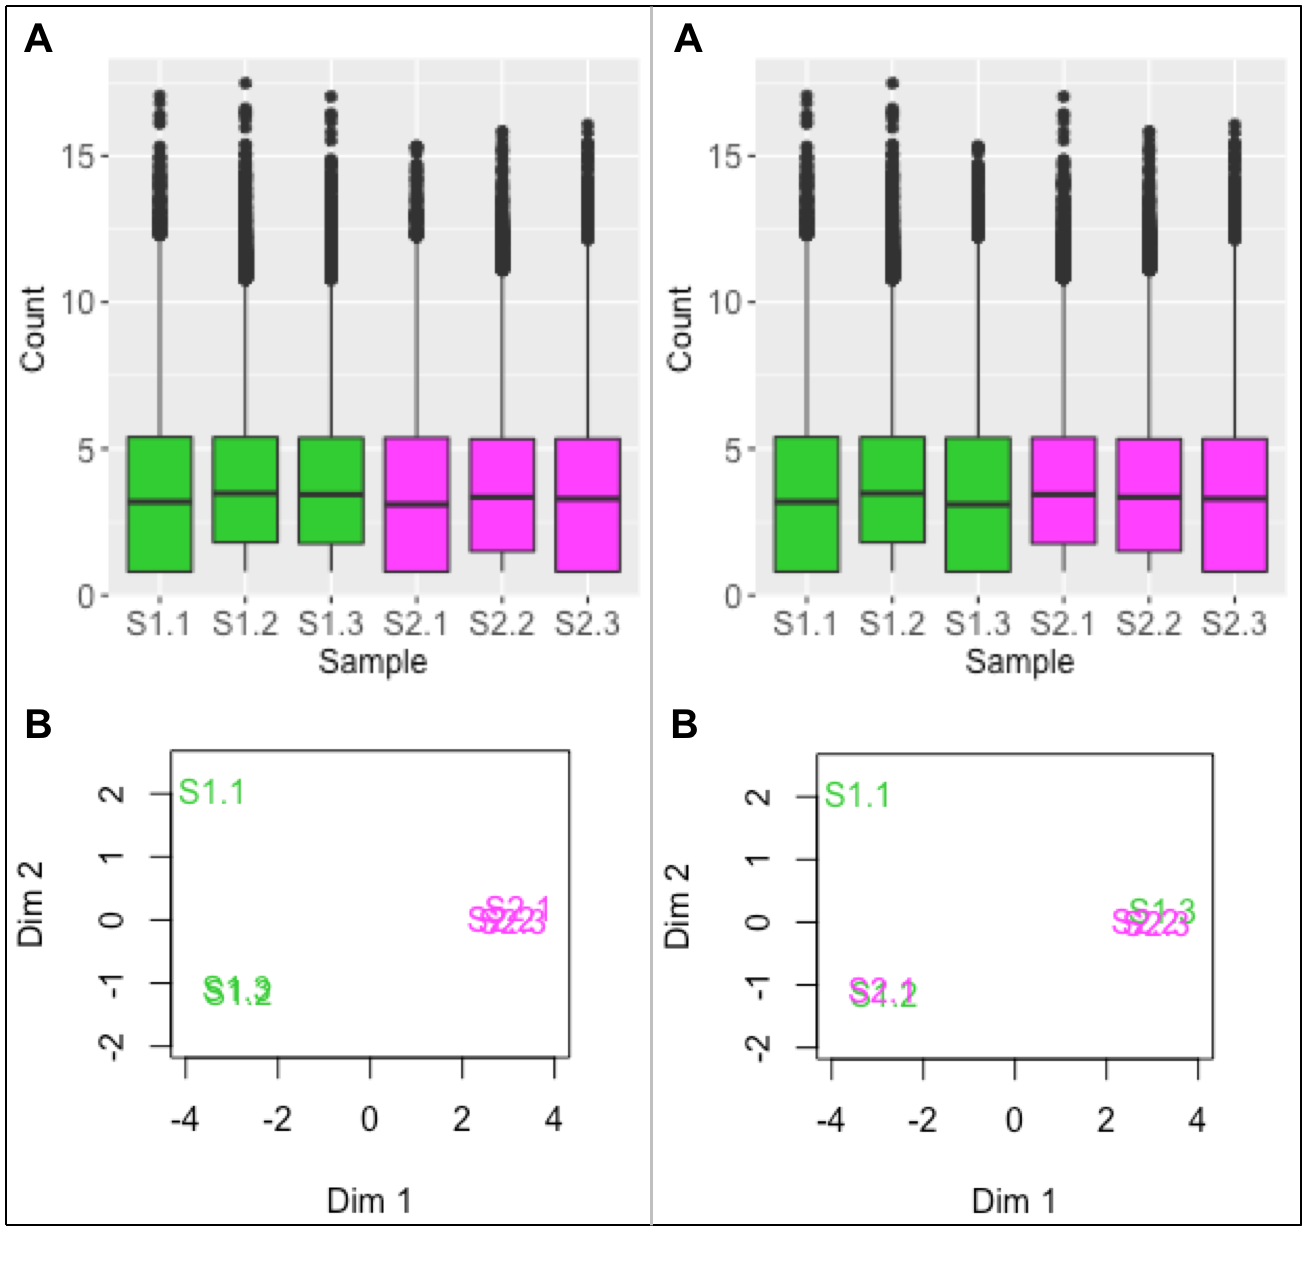
\includegraphics[scale=0.38]{images/mdsSwitch.png}
\end{figure}
\end{frame}

\begin{frame}{}
\begin{figure}
\centering
\fbox{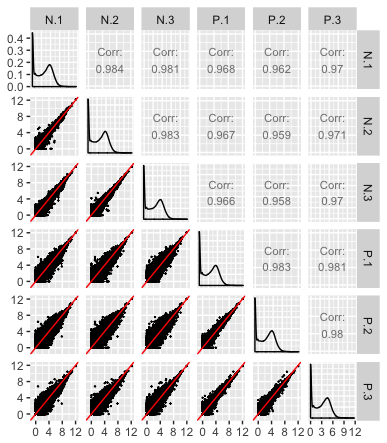
\includegraphics[scale=0.49]{images/sbIRStreak.jpg}}
\end{figure}
\end{frame}

\begin{frame}{}
\begin{figure}
\centering
\fbox{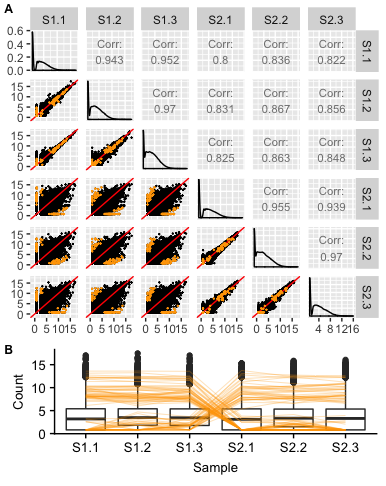
\includegraphics[scale=0.44]{images/sbIRDEG.jpg}}
\end{figure}
\end{frame}

\begin{frame}{}
\begin{figure}
\centering
\fbox{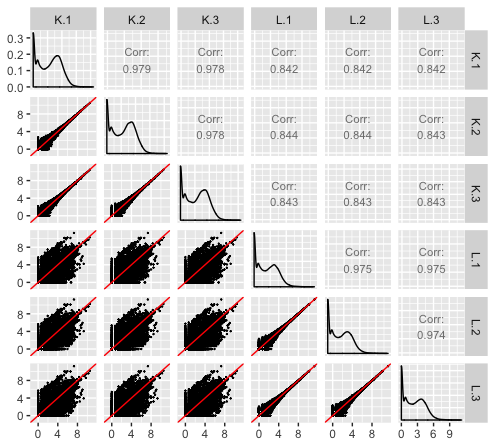
\includegraphics[scale=0.44]{images/lkSM.jpg}}
\end{figure}
\end{frame}

\begin{frame}{}
\begin{figure}
\centering
\fbox{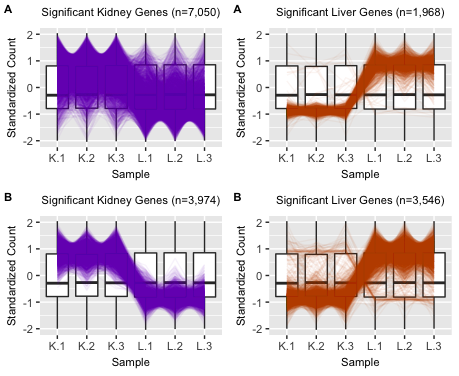
\includegraphics[scale=0.44]{images/lkClusters.jpg}}
\end{figure}
\end{frame}

\begin{frame}{}
\begin{figure}
\centering
\fbox{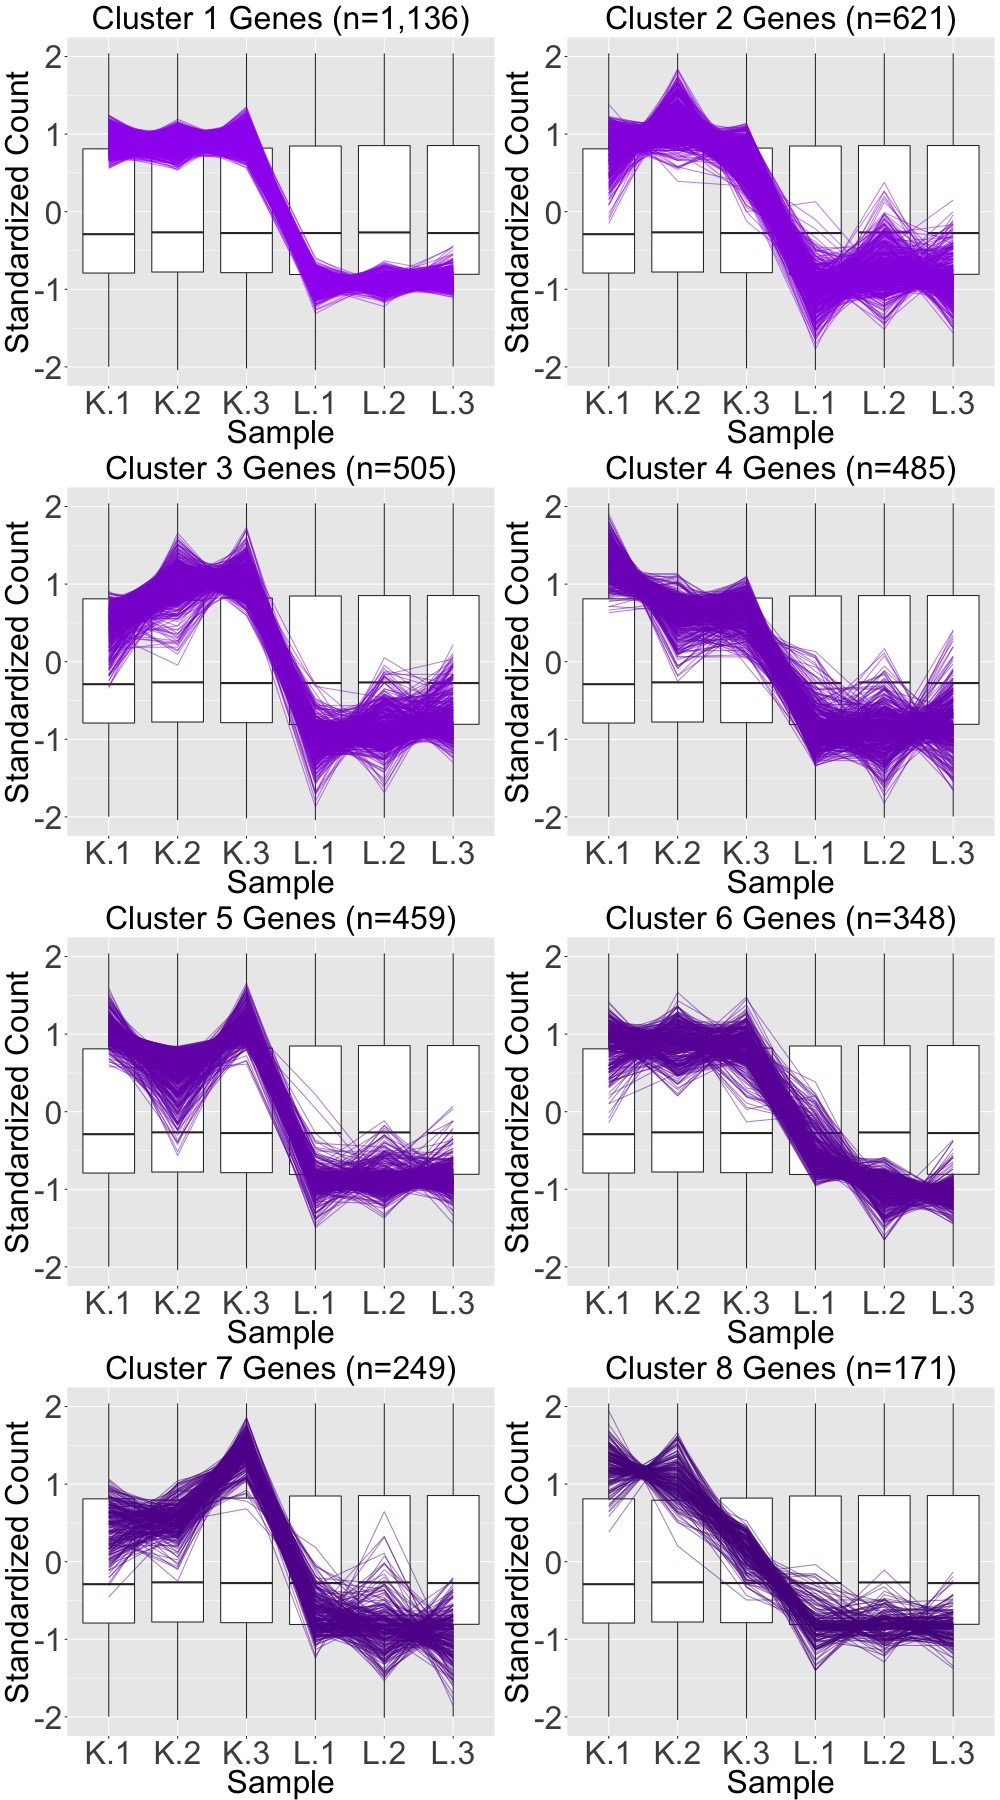
\includegraphics[scale=0.13]{images/lkClustersKeep.jpg}}
\end{figure}
\end{frame}

\begin{frame}{}
\begin{figure}
\centering
\fbox{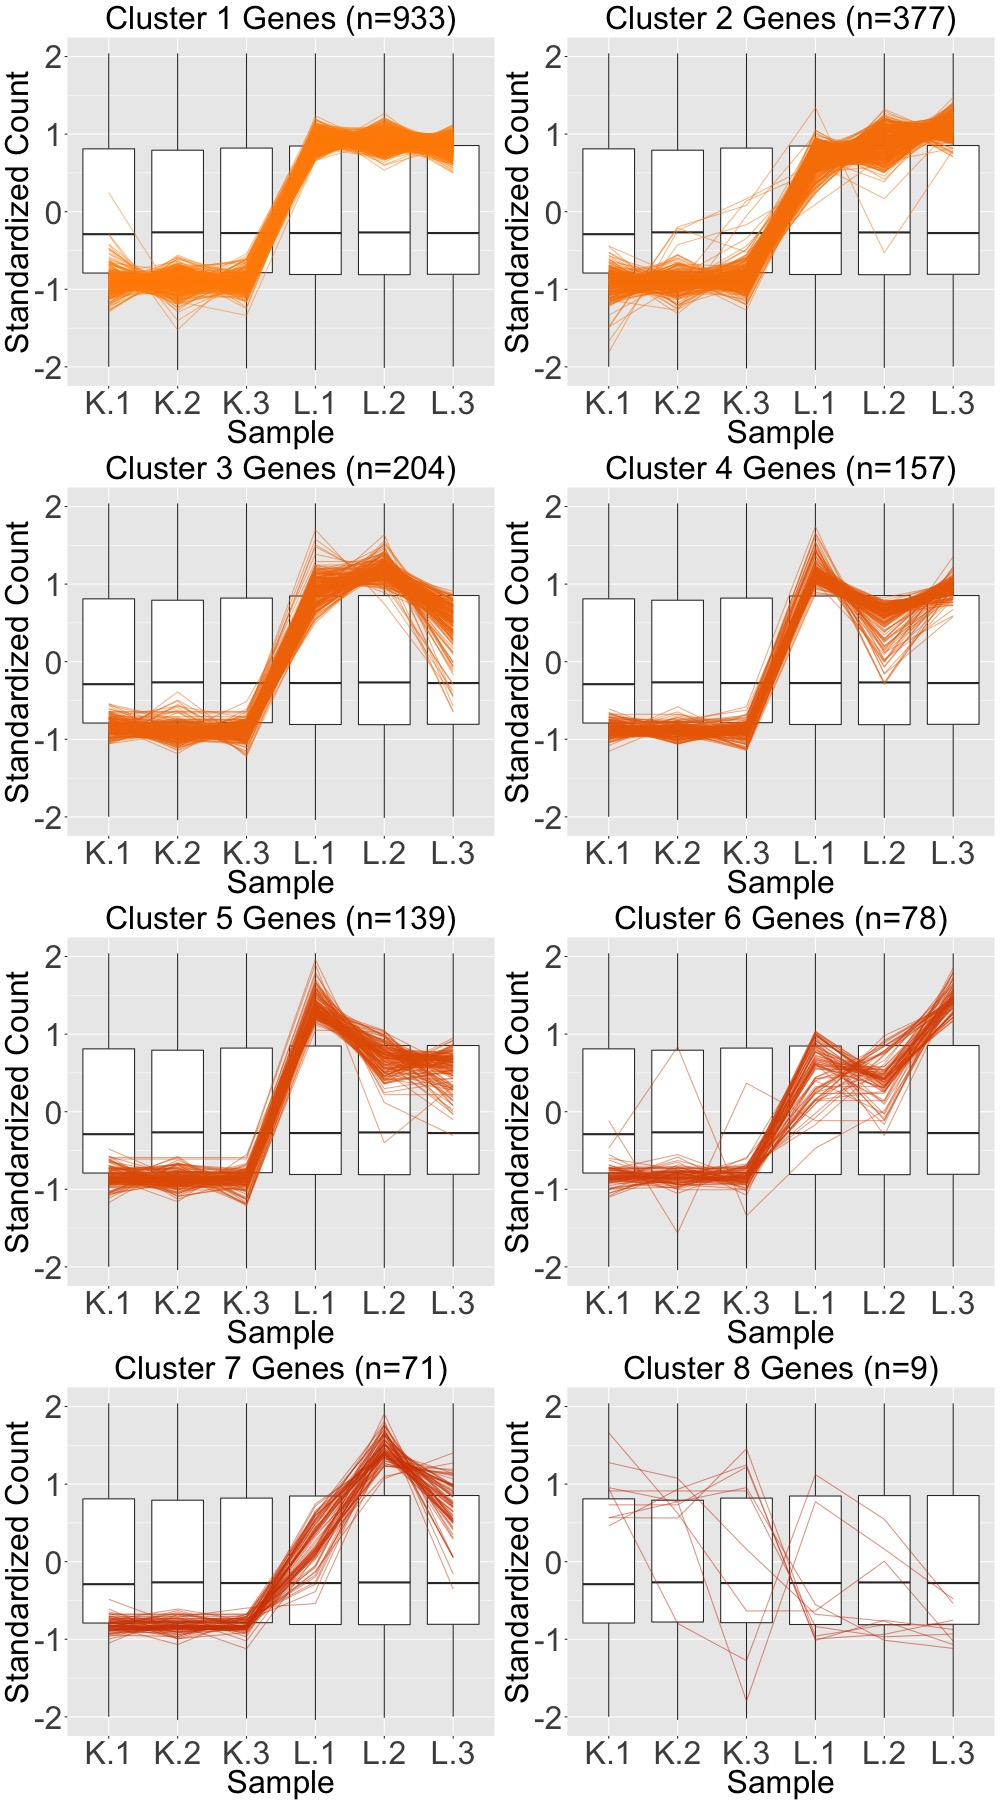
\includegraphics[scale=0.13]{images/lkClustersOrig.jpg}}
\end{figure}
\end{frame}

\begin{frame}{}
\begin{figure}
\centering
\fbox{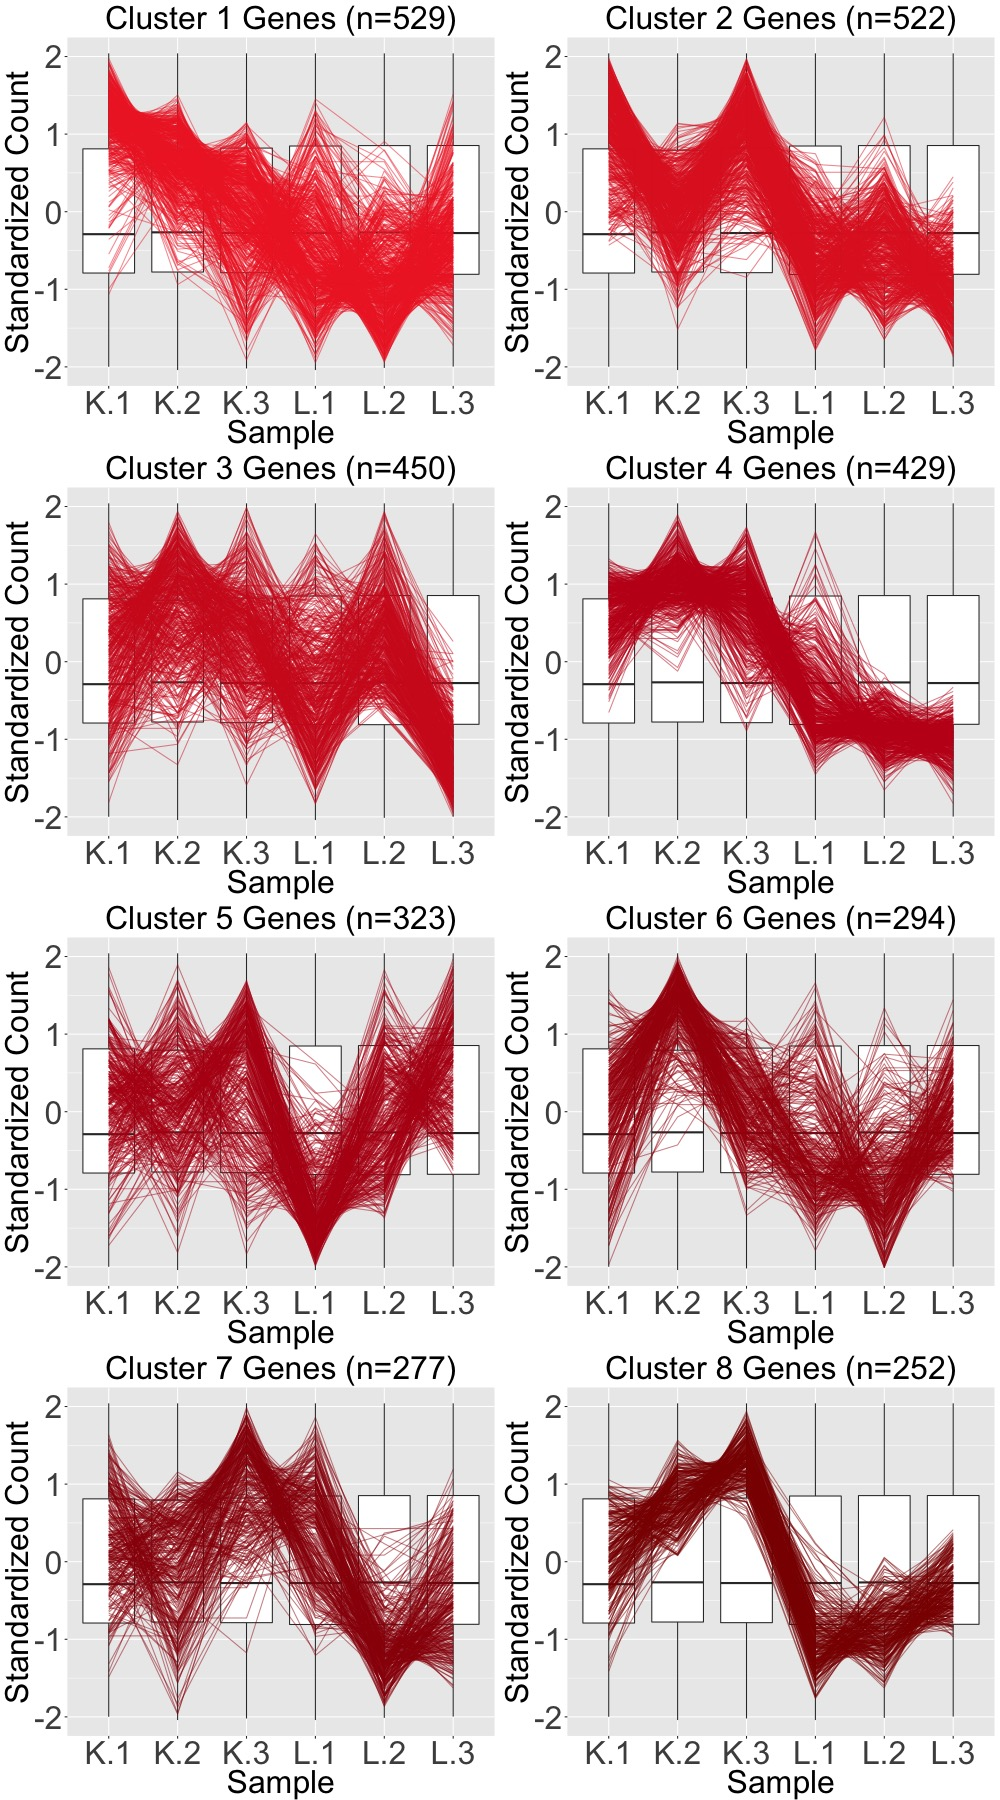
\includegraphics[scale=0.13]{images/lkClustersRemove.jpg}}
\end{figure}
\end{frame}

\begin{frame}{}
\begin{figure}
\centering
\fbox{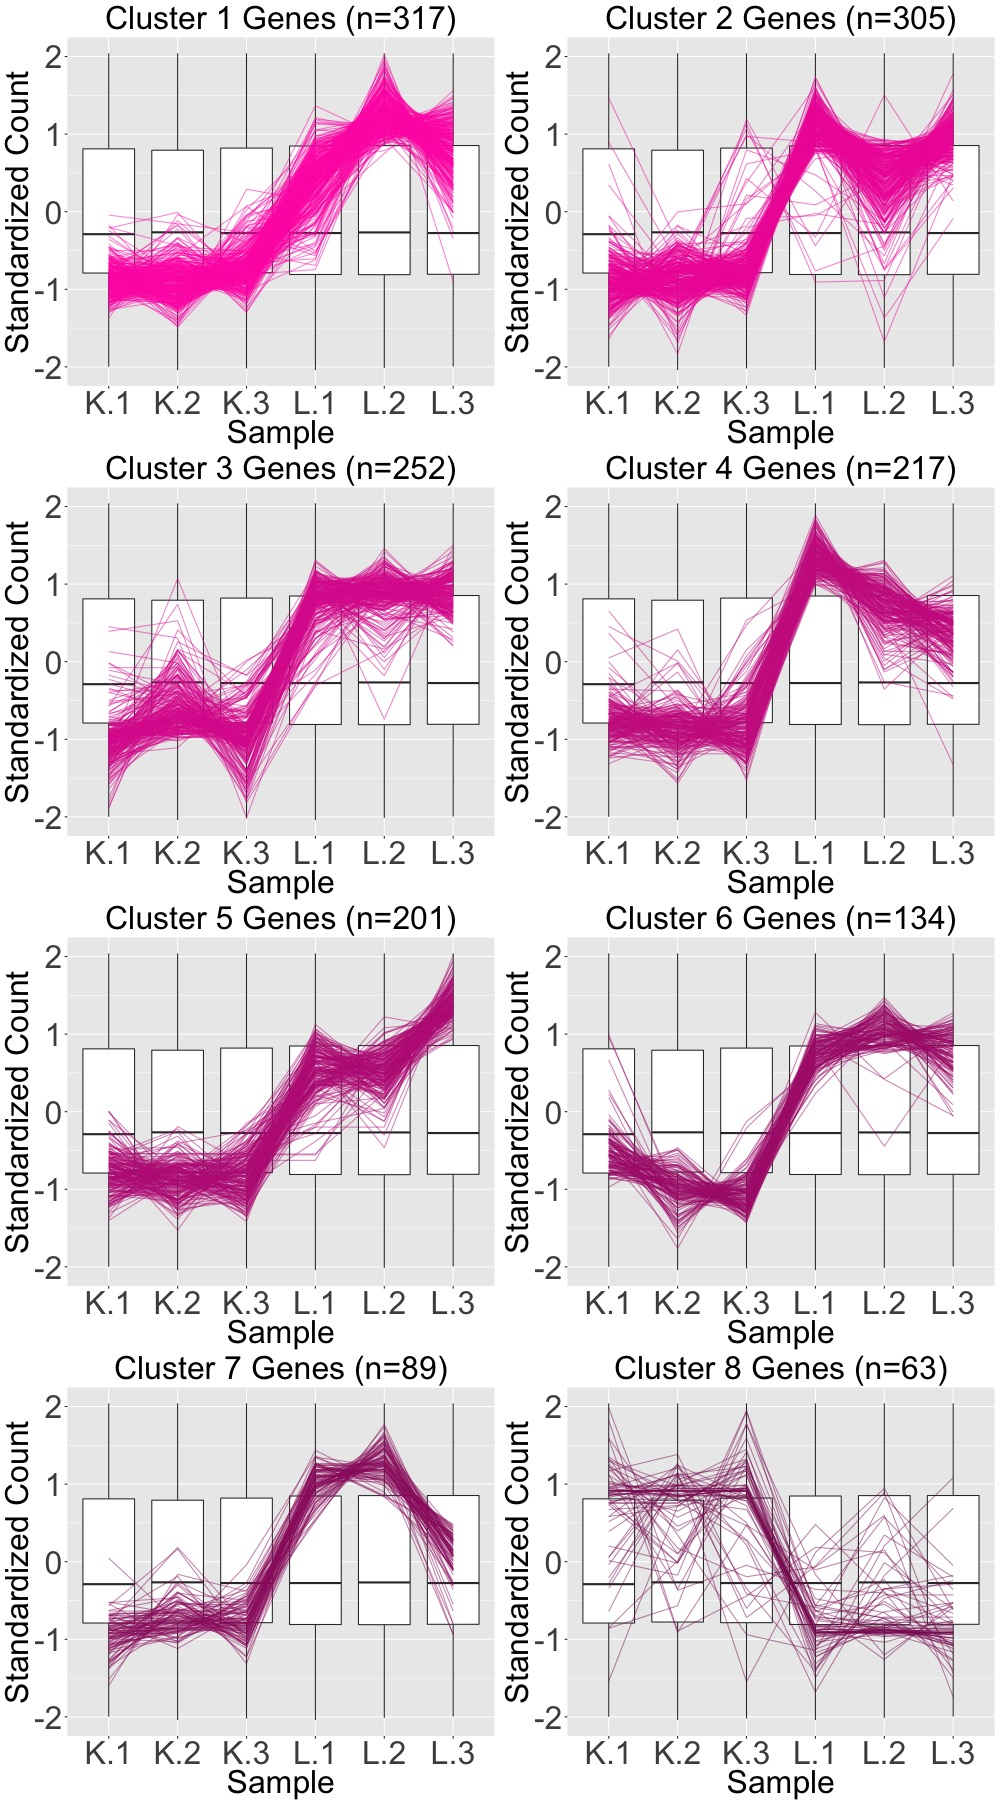
\includegraphics[scale=0.13]{images/lkClustersAdd.jpg}}
\end{figure}
\end{frame}

\begin{frame}{}
\begin{figure}
\centering
\fbox{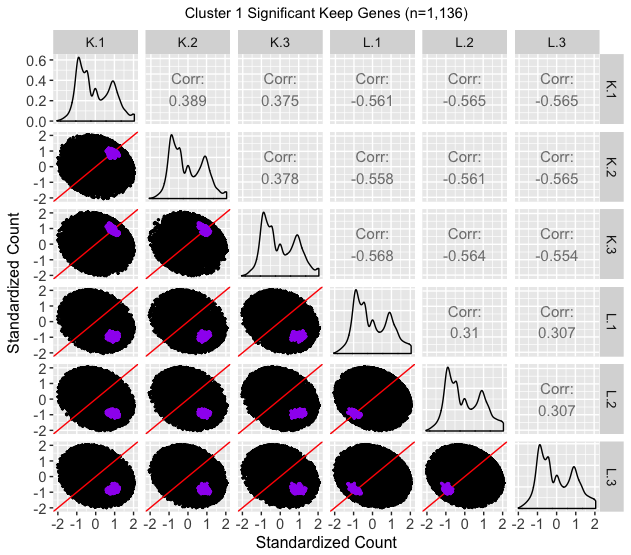
\includegraphics[scale=0.13]{images/lkClustersKeepSM-St.jpg}}
\end{figure}
\end{frame}

\begin{frame}{}
\begin{figure}
\centering
\fbox{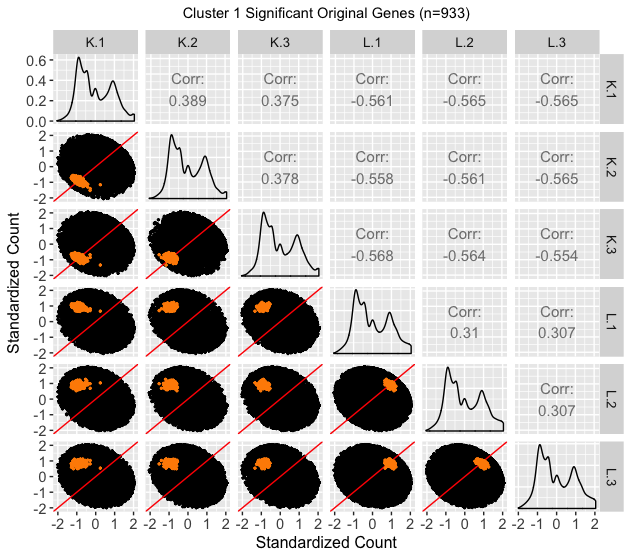
\includegraphics[scale=0.13]{images/lkClustersOrigSM-St.jpg}}
\end{figure}
\end{frame}

\begin{frame}{}
\begin{figure}
\centering
\fbox{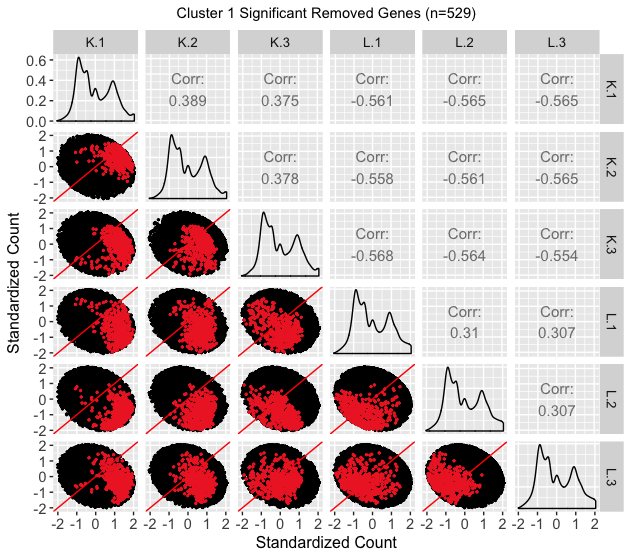
\includegraphics[scale=0.13]{images/lkClustersRemoveSM-St.jpg}}
\end{figure}
\end{frame}

\begin{frame}{}
\begin{figure}
\centering
\fbox{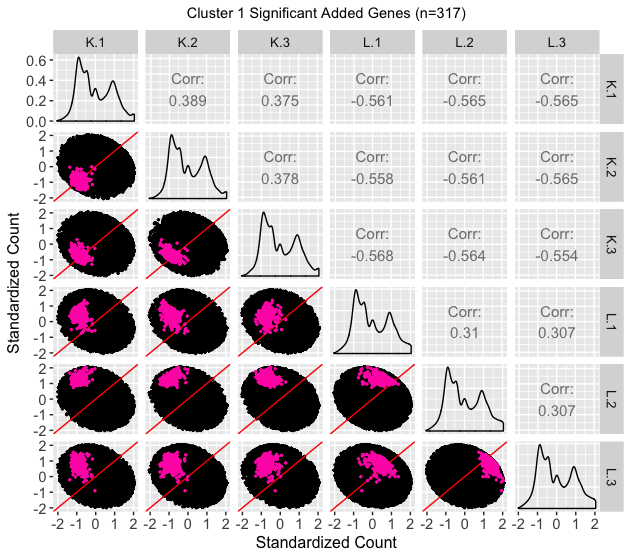
\includegraphics[scale=0.13]{images/lkClustersAddSM-St.jpg}}
\end{figure}
\end{frame}

\begin{frame}{}
\begin{figure}
\centering
\fbox{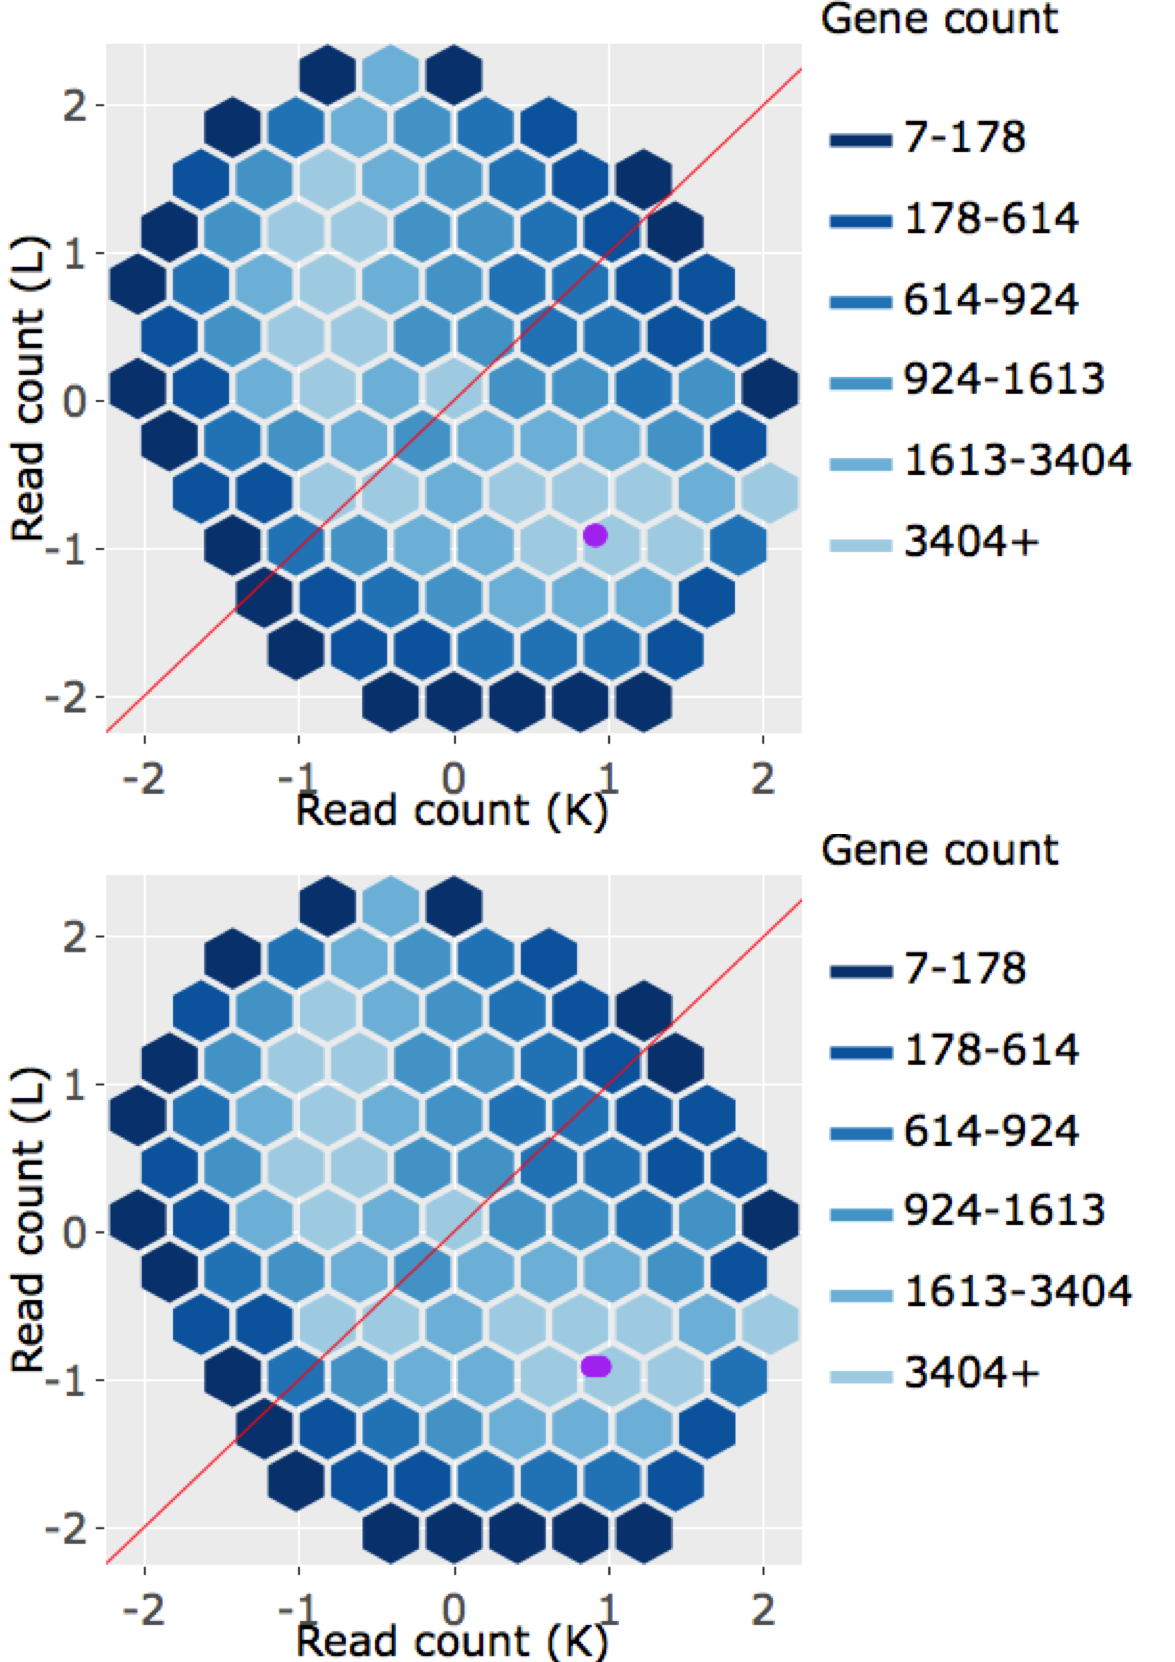
\includegraphics[scale=0.13]{images/litreClusterKeep-St.jpg}}
\end{figure}
\end{frame}

\begin{frame}{}
\begin{figure}
\centering
\fbox{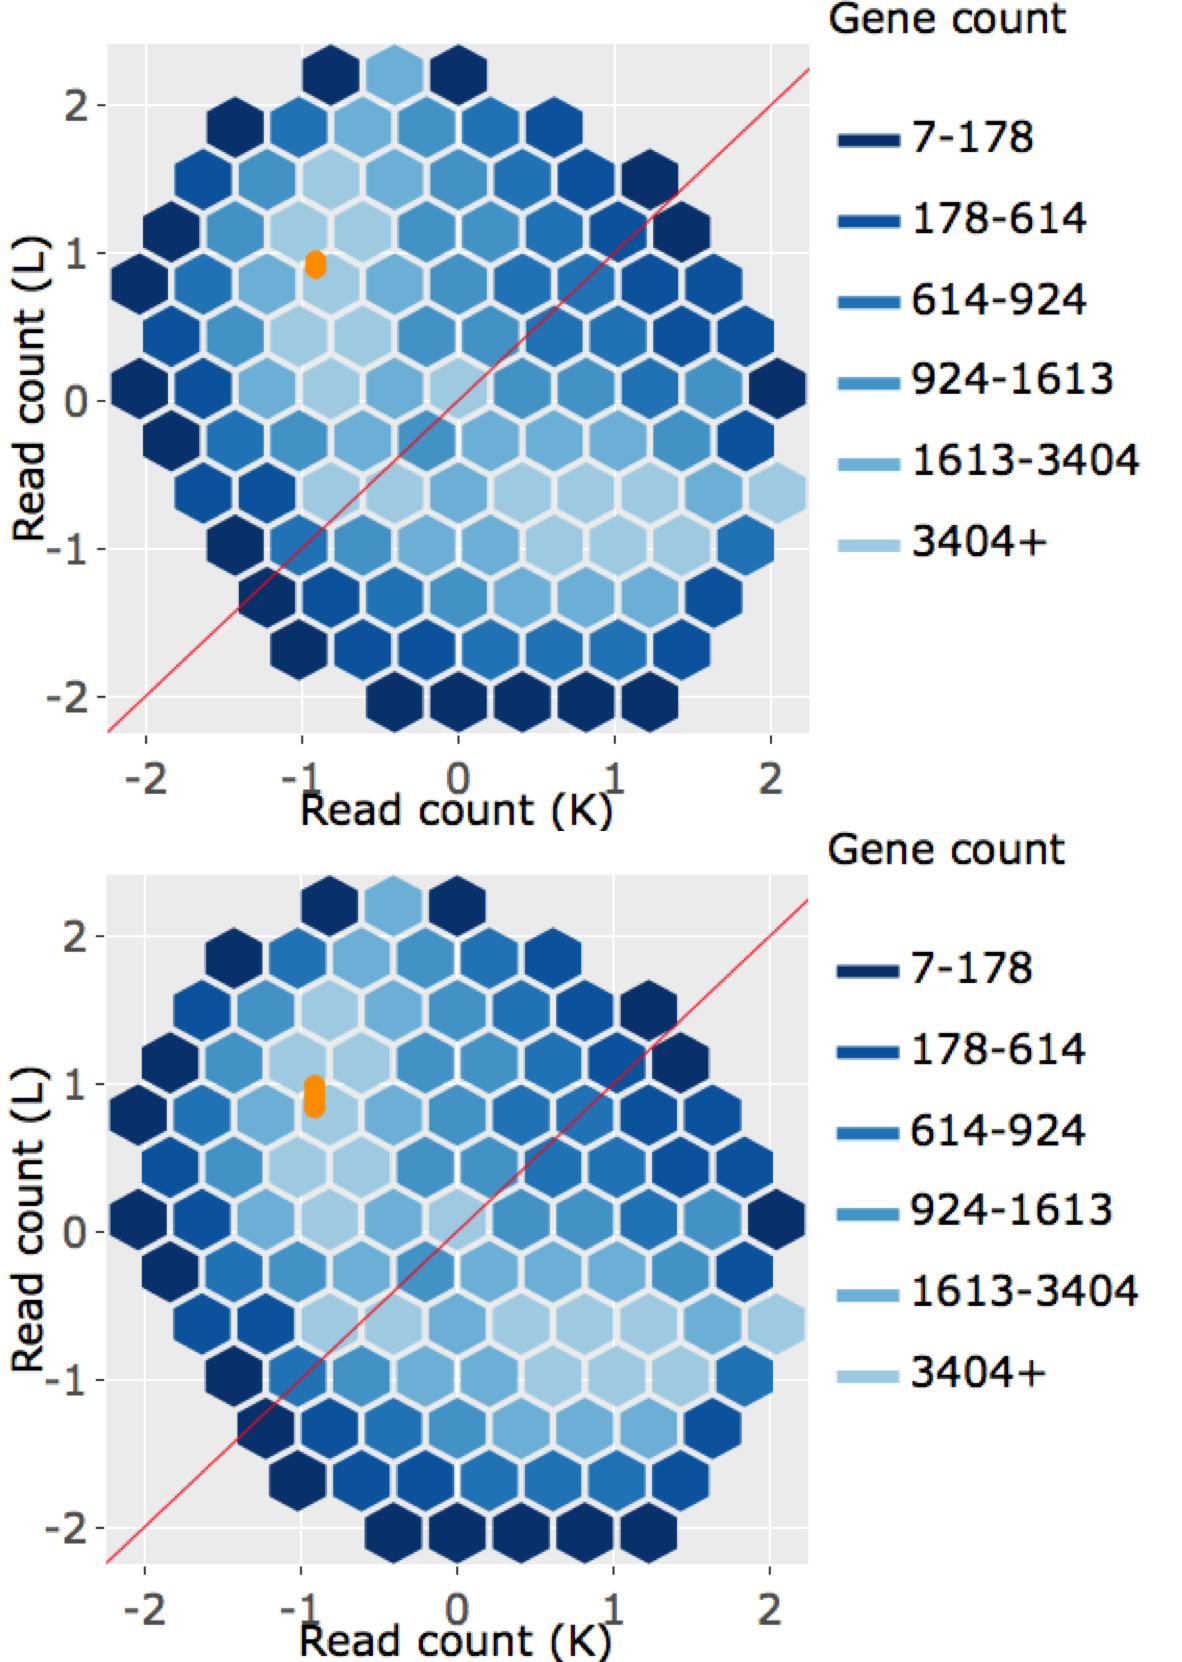
\includegraphics[scale=0.13]{images/litreClusterOrig-St.jpg}}
\end{figure}
\end{frame}

\begin{frame}{}
\begin{figure}
\centering
\fbox{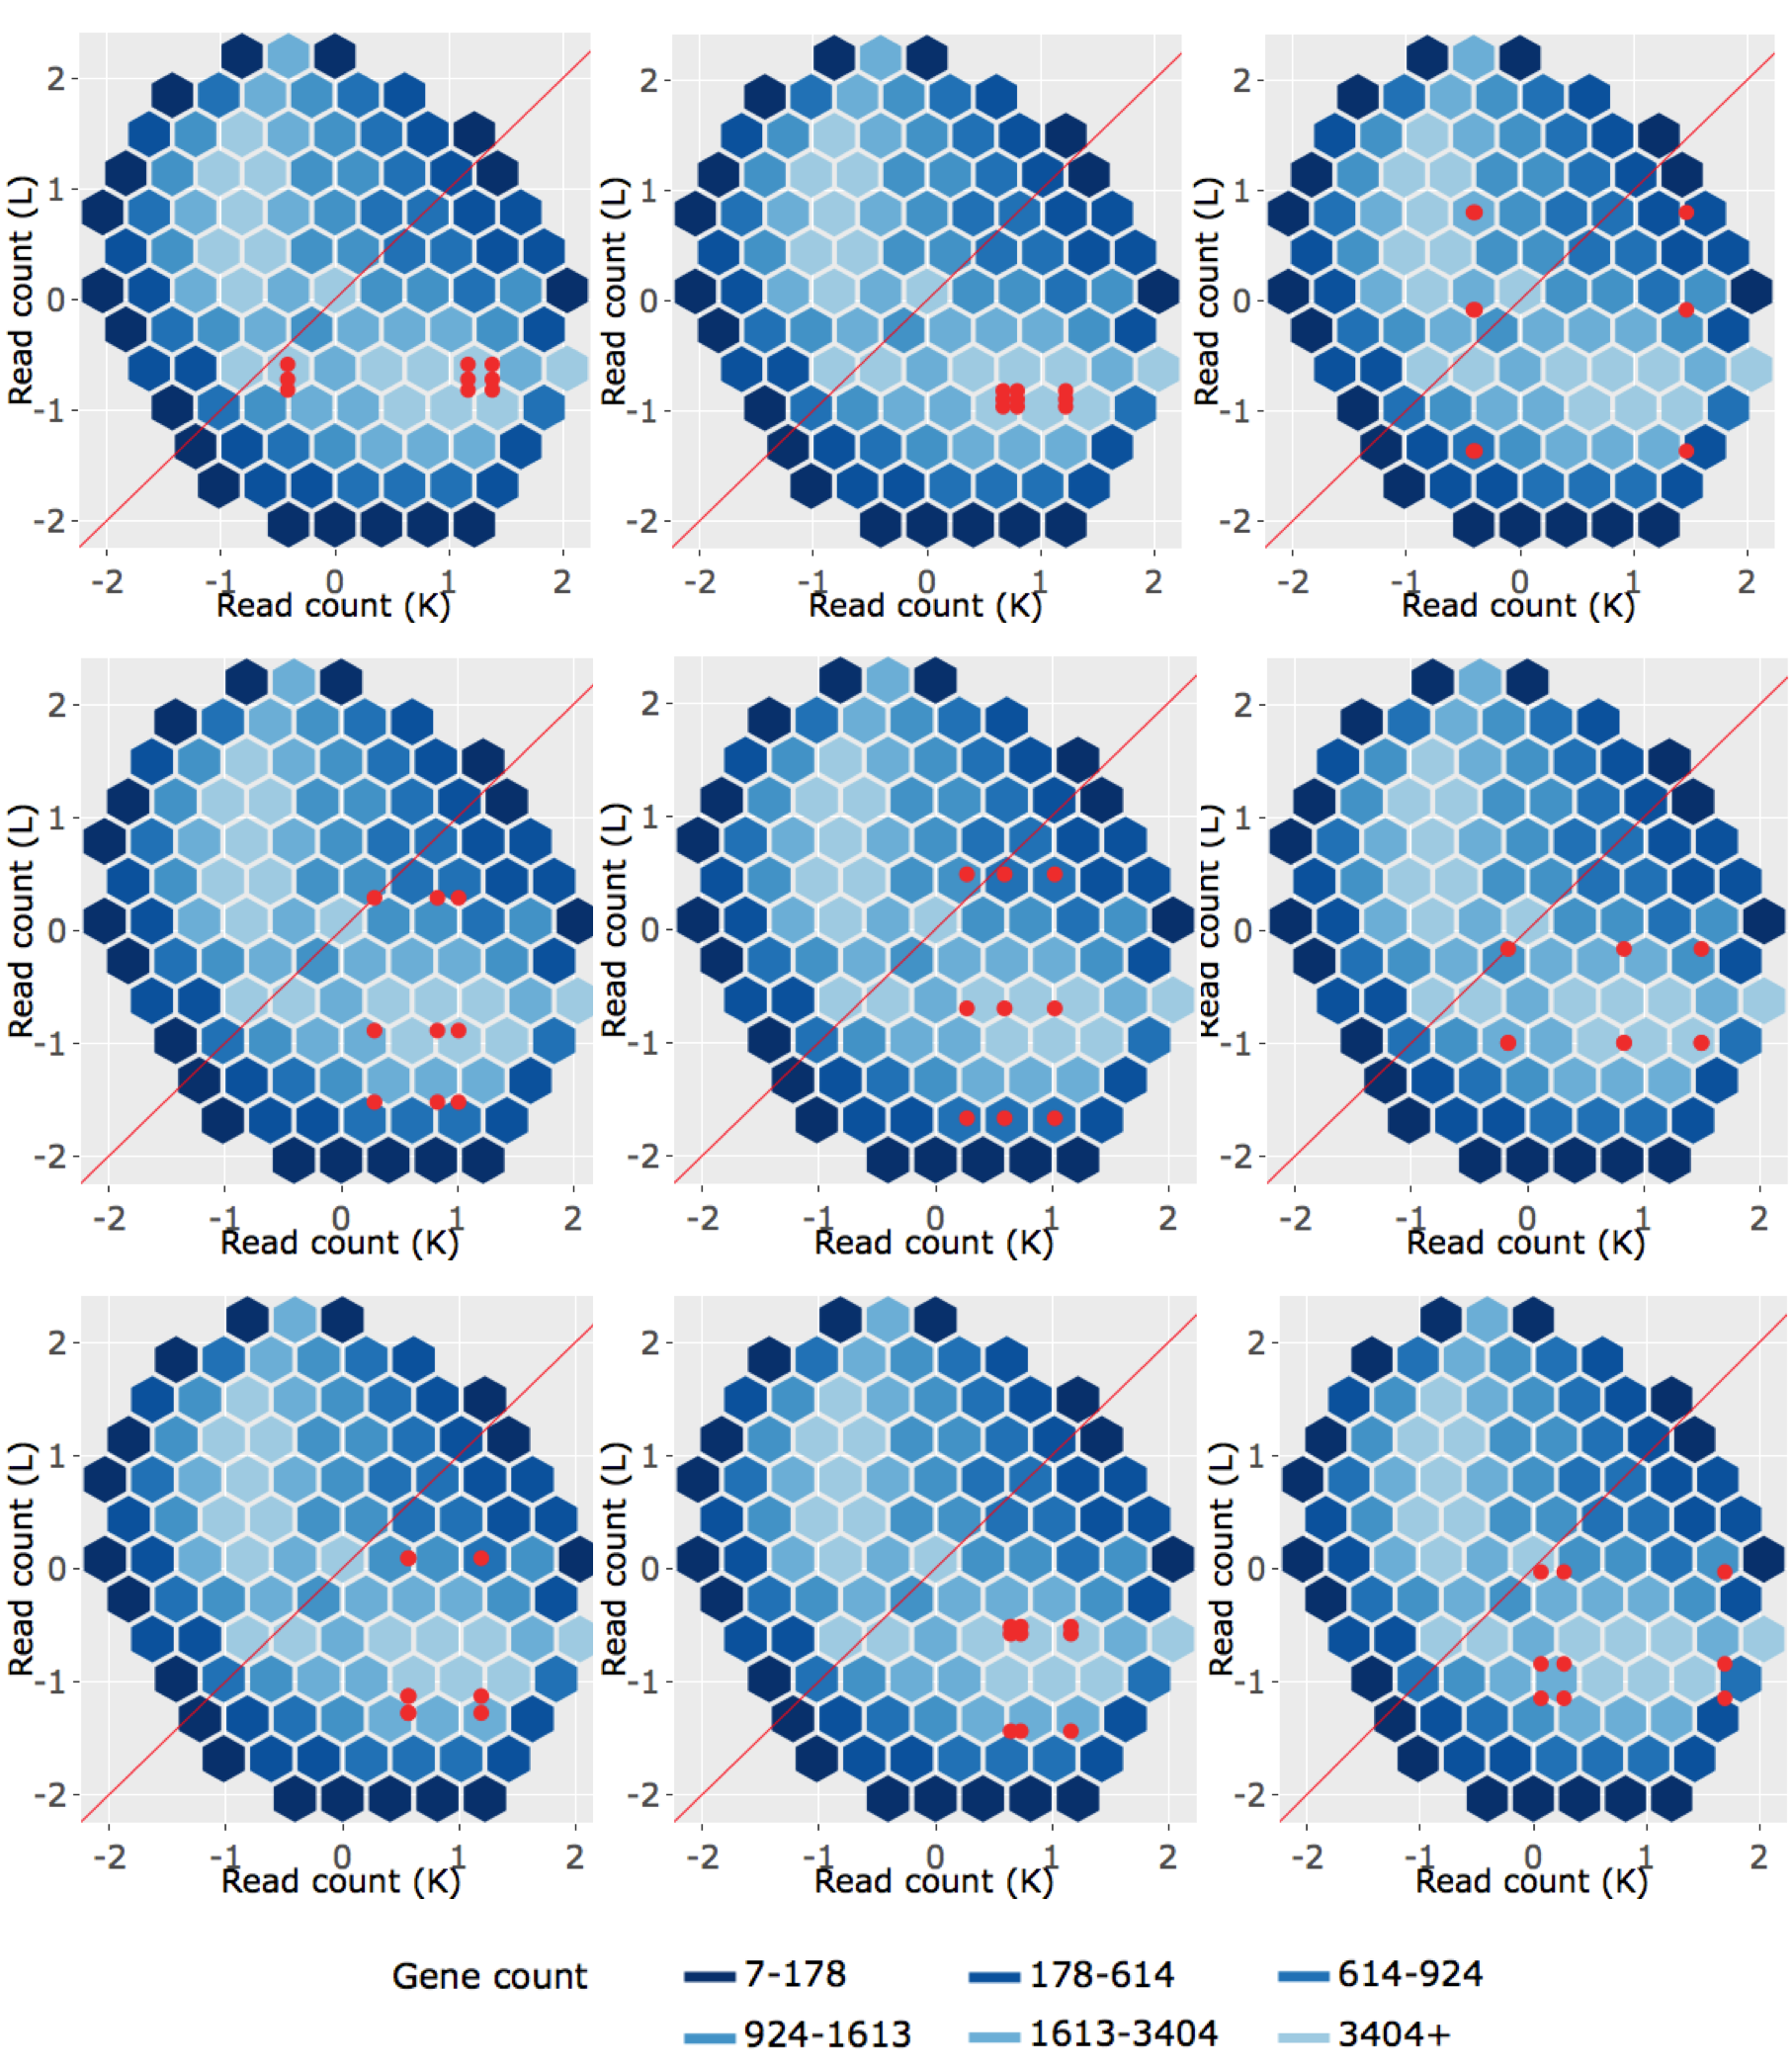
\includegraphics[scale=0.13]{images/litreClusterRemove-St.jpg}}
\end{figure}
\end{frame}

\begin{frame}{}
\begin{figure}
\centering
\fbox{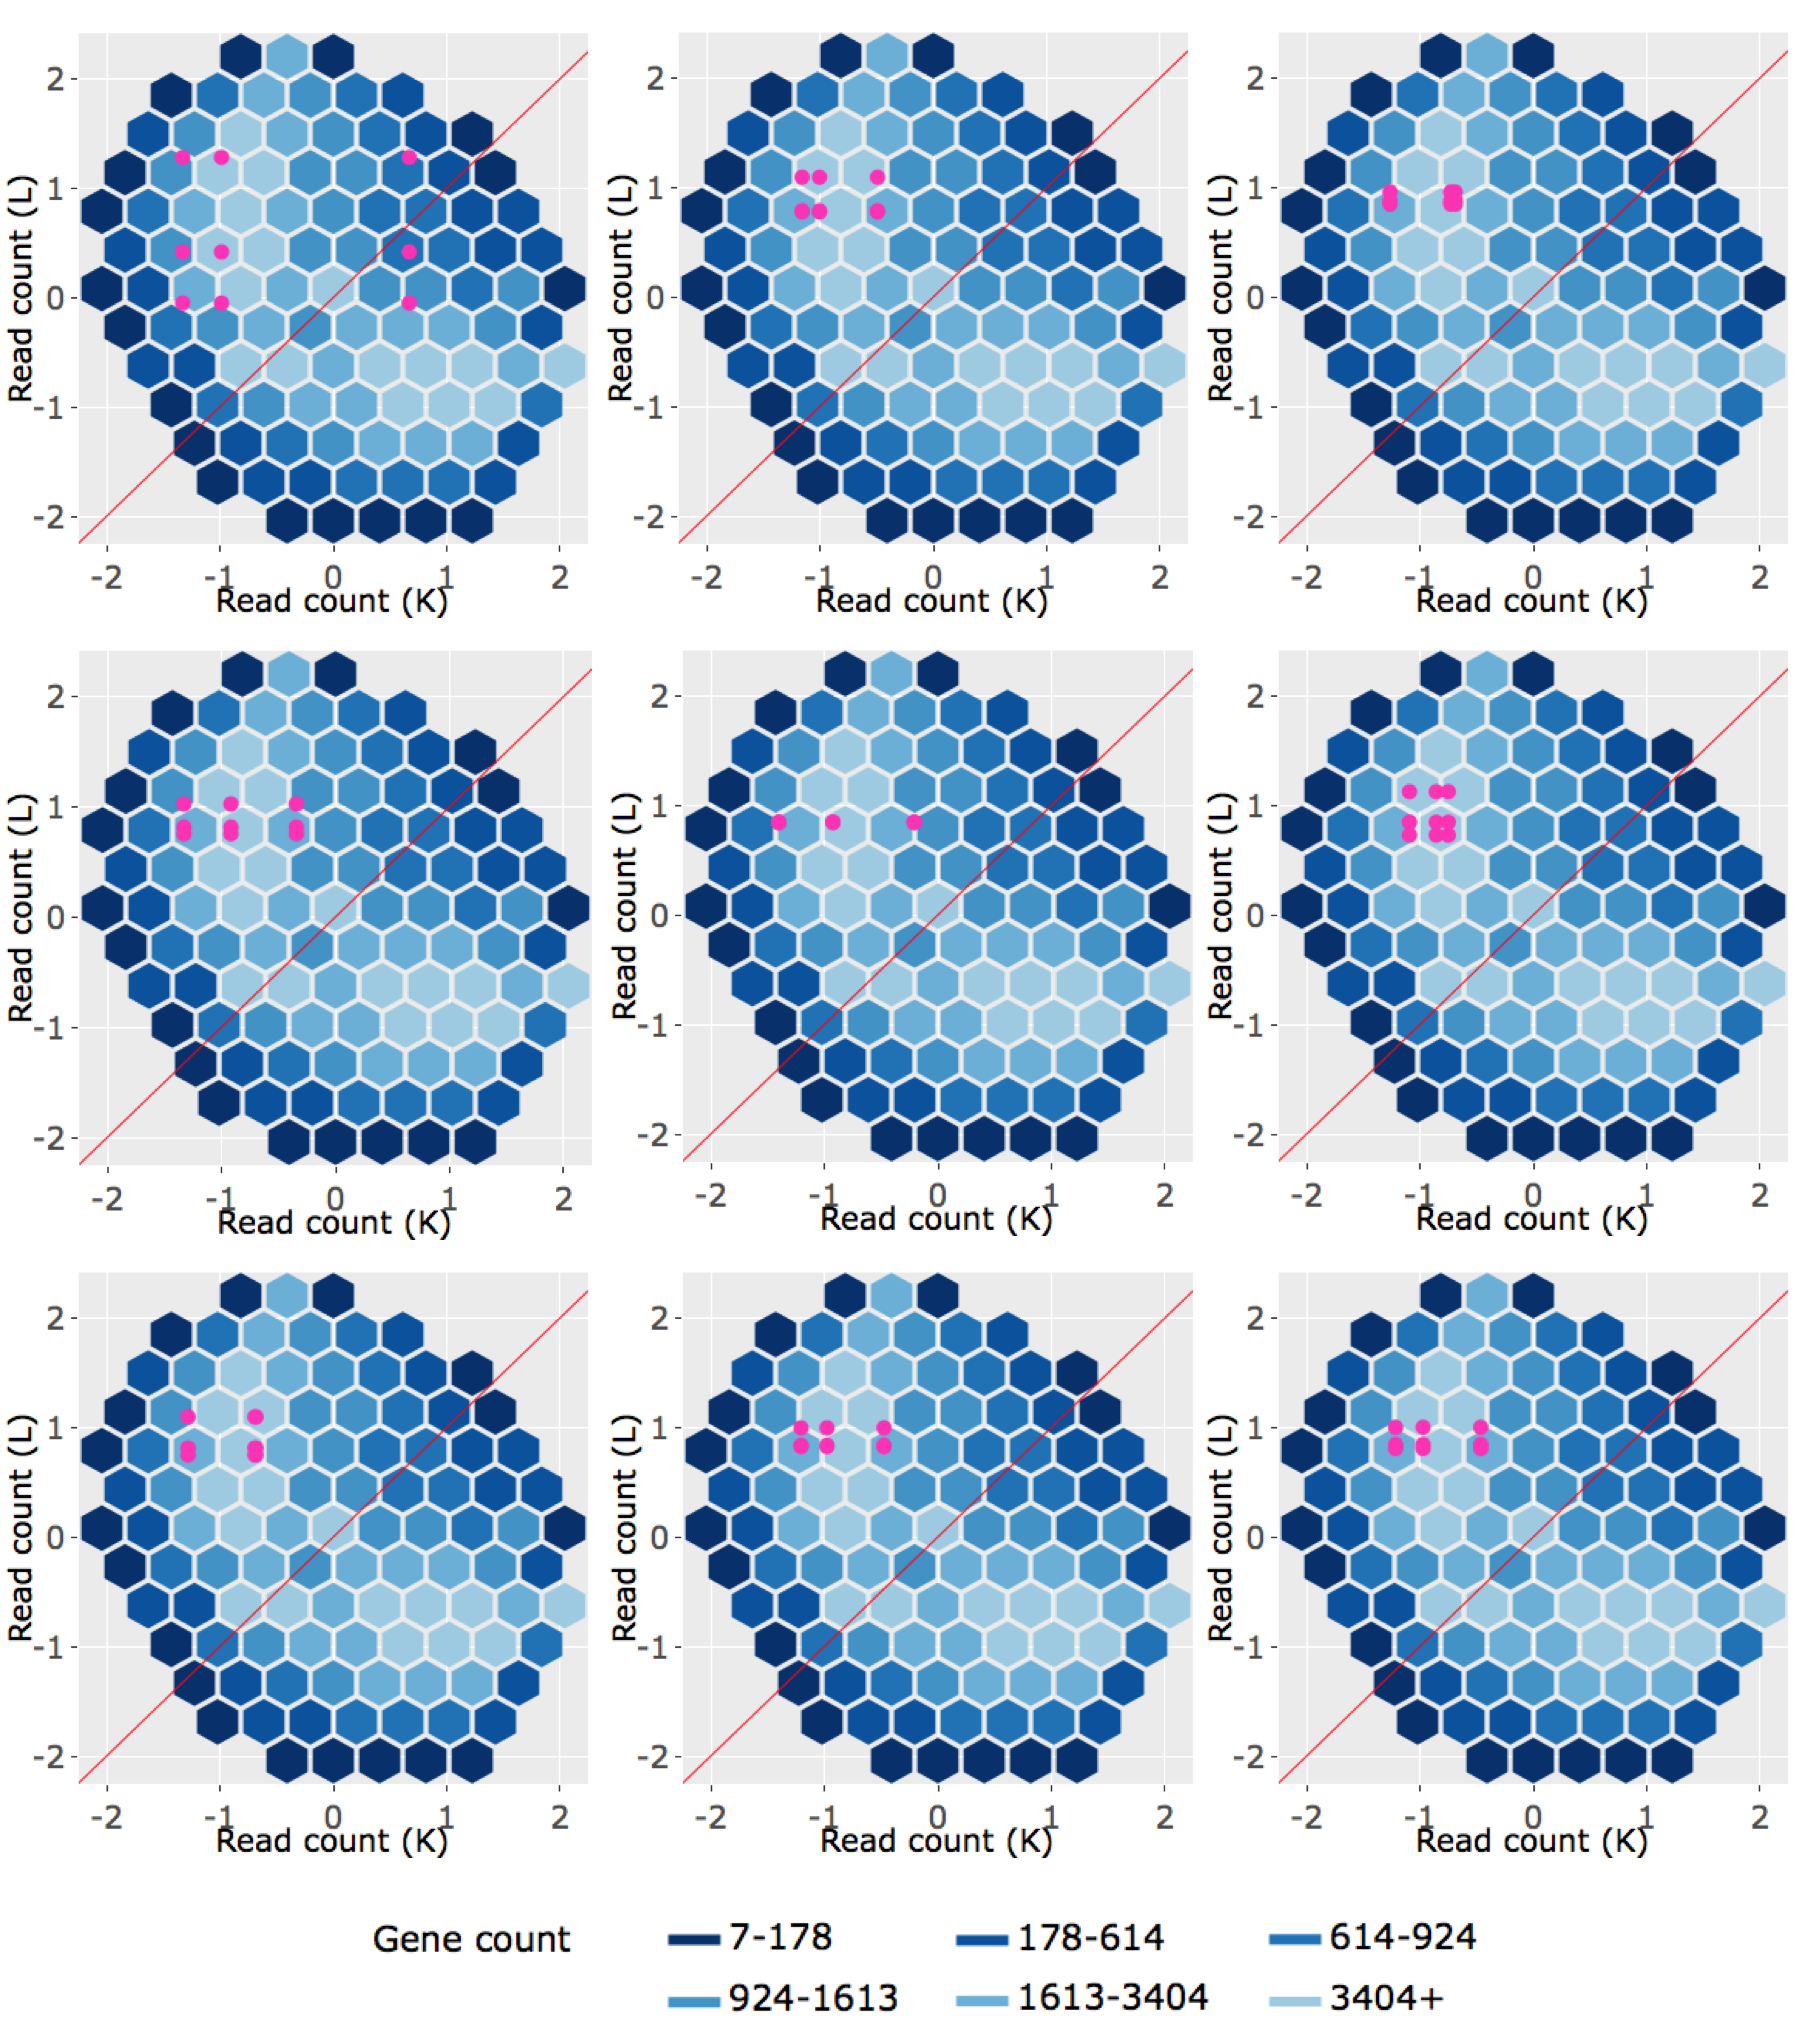
\includegraphics[scale=0.13]{images/litreClusterAdd-St.jpg}}
\end{figure}
\end{frame}






%%%%%%%%%%%%%%%%%%%%%%%%%%%%%%%%% TIMELINE %%%%%%%%%%%%%%%%%%%%%%%%%%%%%
\section{Timeline}

\begin{frame}{Completed work}
\begin{tabular}{|p{1.5cm}|p{5.5cm}|p{1.8cm}|}
 \hline
 \textbf{Product} & \textbf{Description} & \textbf{Date} \\ 
 \hline
 R package & First release of \texttt{ggenealogy}, which provides visualization tools for genealogical datasets & March 2015 \\
 \hline
 Presentation & Presented \texttt{ggenealogy} at JSM & August 2015 \\
 \hline
 Award & Student paper award at ASA Statistical Computing and Graphics Section & August 2015 \\
 \hline
\end{tabular}
\end{frame}

\begin{frame}{Scheduled deliverables}
\begin{tabular}{|p{1.5cm}|p{5.5cm}|p{1.8cm}|}
 \hline
 \textbf{Product} & \textbf{Description} & \textbf{Date} \\ 
 \hline
 R package & Second release of \texttt{ggenealogy} package, which provides visualization tools for genealogical datasets & May 2016 \\
 \hline
 Paper & Submit \texttt{ggenealogy} paper to JSS & May 2016 \\
 \hline
 R package & First release of package that provides visualization tools for RNA-sequencing datasets & TBD \\
 \hline
 Paper & Submit paper about visualization tools for clustering analysis of RNA-sequencing & TBD \\
 \hline
 Paper & Submit paper about visualization tools for significance testing of RNA-sequencing & TBD \\
 \hline
\end{tabular}
\end{frame}

\begin{frame}{Other work}
\begin{tabular}{|p{1.5cm}|p{5.5cm}|p{1.8cm}|}
 \hline
 \textbf{Product} & \textbf{Description} & \textbf{Date} \\ 
 \hline
 R package & First release of ePort package that generates electronic reports for instructors to evaluate student performance & July 2016 \\
 \hline
\end{tabular}
\end{frame}

\begin{frame}{References}
  \begin{itemize}
    \item \texttt{ggplot2} (Wickham 2009)
    \item \texttt{GGally} (Schloerke et al. 2016)
    \item \texttt{nullabor} (Wickham et al. 2014)
    \item \texttt{ggbio} (Yin et al. 2012)
    \item \texttt{GGobi} (Swayne et al. 2003)
    \item \texttt{tourr} (Wickham et al. 2011)
    \item \texttt{plotly} (Sievert et al. 2016)
    \item Parallel coordinate plots (Inselberg 1985, Wegman 1990)
    \item Visual statistical inference (Chowdhury et al. 2015)
	\end{itemize}
\end{frame}

\begin{frame}{References}
  \begin{itemize}
    \item \texttt{pedigree} (Coster 2013)
    \item \texttt{kinship2} (Therneau et al. 2015)
    \item \texttt{GraphViz} (Gansner and North 2000)
    \item \texttt{Cytoscape} (Shannon et al. 2003)
    \item \texttt{explorase} (Lawrence et al. 2008)
    \item \texttt{edgeR} (Robinson et al. 2010)
    \item \texttt{DESeq2} (Love at al. 2014)
    \item \texttt{RUVseq} (Risso et al. 2014)
    \item Gene expression visual inference (Yin et al. 2013)
    \item Biological clustering: (Newell et al. 2013)
	\end{itemize}
\end{frame}

%%%%%%%%%%%%%%%%%%%%%%%%%%%%%%%%% EXTRA %%%%%%%%%%%%%%%%%%%%%%%%%%%%%
\begin{frame}{Leaves at 120 minutes - 3 Clusters}
% \begin{figure}
% \centering
% \fbox{\includegraphics[scale=0.65]{indSBGenes2.png}}
% \end{figure}
\end{frame}
\end{document}
